\listfiles
\documentclass[5p,times]{elsarticle}

\usepackage{lineno,hyperref}
\usepackage{booktabs}
\modulolinenumbers[5]
\usepackage{color}
\usepackage{comment}
\usepackage{verbatim}


%%%%%%%%%%%%%%%%%%%%%%%
%% Elsevier bibliography styles
%%%%%%%%%%%%%%%%%%%%%%%
%% To change the style, put a % in front of the second line of the current style and
%% remove the % from the second line of the style you would like to use.
%%%%%%%%%%%%%%%%%%%%%%%

% Numbered
% \bibliographystyle{model1-num-names}

%% Numbered without titles
% \bibliographystyle{model1a-num-names}

%% Harvard
% \bibliographystyle{model2-names}\biboptions{authoryear}

%% Vancouver numbered
% \usepackage{numcompress}\bibliographystyle{model3-num-names}

%% Vancouver name/year
% \usepackage{numcompress}\bibliographystyle{model4-names}\biboptions{authoryear}

%% APA style
% \bibliographystyle{model5-names}\biboptions{authoryear}

%% AMA style
% \usepackage{numcompress}\bibliographystyle{model6-num-names}

%% `Elsevier LaTeX' style, distributed in TeX Live 2019
\bibliographystyle{elsarticle-num}
% \usepackage{numcompress}\bibliographystyle{elsarticle-num-names}
% \bibliographystyle{elsarticle-harv}\biboptions{authoryear}
%%%%%%%%%%%%%%%%%%%%%%%

\newif\ifargonnereport
\argonnereportfalse
\newif\iffinal
\finalfalse

\iffinal
  \newcommand\todd[1]{}
  \newcommand\todo[1]{}
\else 
  \definecolor{puce}{rgb}{0.8,0.53,0.6}
  \newcommand\todd[1]{\textcolor{puce}{Todd: #1}}
  \newcommand\todo[1]{\textcolor{red}{Todo: #1}}
\fi 



\begin{document}

%\ifargonnereport
%\onecolumn
\pagestyle{empty}

\vspace{1.75in}

\begin{centering}

ARGONNE NATIONAL LABORATORY

9700 South Cass Avenue

Argonne, Illinois  60439

\vspace{1.5in}

{\large \textbf{Toward Performance-Portable PETSc for GPU-based Exascale Systems}}

\vspace{.5in}

\textbf{Richard Tran Mills, Mark F. Adams, Satish Balay, Jed Brown, Alp Dener, Matthew Knepley, Scott E. Kruger, Hannah Morgan, Todd Munson, Karl Rupp, Barry F. Smith, Stefano Zampini, Hong Zhang, Junchao Zhang}

\vspace{.5in}

%% Argonne Leadership Facility and
Mathematics and Computer Science Division

\vspace{.25in}

Preprint ANL/MCS-P9401-1020

\vspace{.5in}

October 2020

\end{centering}

\vspace{2.0in}

\bigskip

\par\noindent
\footnotetext [1]
{
This work was supported by the Exascale Computing Project (17-SC-20-SC), a collaborative 
effort of two US Department of Energy organizations (Office of Science and the National
Nuclear Security Administration), responsible for the planning and preparation
of a capable exascale ecosystem, including software, applications, hardware,
advanced system engineering, and early testbed platforms, in support of the
nation’s exascale computing imperative, and by the Austrian Science Fund (FWF) under grant P29119-N30.  This research used resources of the 
Argonne and Oak Ridge Leadership Computing Facilities, DOE Office of Science 
User Facilities supported under Contracts DE-AC02-06CH11357 and 
DE-AC05-00OR22725, respectively.
}

\newpage

\vspace*{\fill}
\begin{center}
\fbox{
\parbox{4in}{
The submitted manuscript has been created by UChicago Argonne, LLC, Operator of Argonne
National Laboratory (``Argonne''). Argonne, a U.S. Department of Energy Office of Science
laboratory, is operated under Contract No. DE-AC02-06CH11357. The U.S. Government retains
for itself, and others acting on its behalf, a paid-up nonexclusive, irrevocable worldwide
license in said article to reproduce, prepare derivative works, distribute copies to the
public, and perform publicly and display publicly, by or on behalf of the Government.
The Department of Energy will provide public access to these results of federally
sponsored research in accordance with the DOE Public Access
Plan. \url{http://energy.gov/downloads/doe-public-accessplan}
}}
\end{center}
\vfill

\newpage
\pagestyle{plain}
\setcounter{page}{1}

%\fi

\begin{frontmatter}

\title{PETSc's Algebraic multigrid solver on GPUs}

%\begin{abstract}
%\end{abstract}

\author[lbnl-address]{Mark F. Adams}

\address[lbnl-address]{Lawrence Berkeley National Laboratory, Berkeley CA 94720 USA}
\end{frontmatter}

%------------------------------------------

% PETSc supports several GPU targets as shown in Figure \ref{fig:petsc_backends-kokkos}.
PETSc's native algebraic multigrid (AMG) solver uses standard sparse numerical kernels and vector operations and, as such, can run entirely on the GPU in the solve phase with relative ease.
Common sparse numerical kernels are provided by third party libraries from vendors such as cuSparse, or others such as Kokkos kernels.
This ability to abstract the AMG algorithm with standard sparse linear algebra has facilitated AMG's widespread use in the PETSc and wider computational science community.
PETSc's linear algebra is built on shared memory matrix and vector objects, which have multiple back-ends for portability.

These objects are composed with a portable C/MPI layer to provide a complete scalable solver.
This MPI layer supports, in general, multiple ``GPU aware MPI" back-ends for portability, which allows the data to reside entirely on the GPU for the entire solves phase, after the setup phase, which is not to date performed on the GPU.
We are developing GPU implementations of parts of the setup phase of AMG, such as the maximal independent set algorithm for graph coarsening and the matrix triple product for Galerkin coarse grid construction.

\begin{figure}[htbp]
\begin{center}
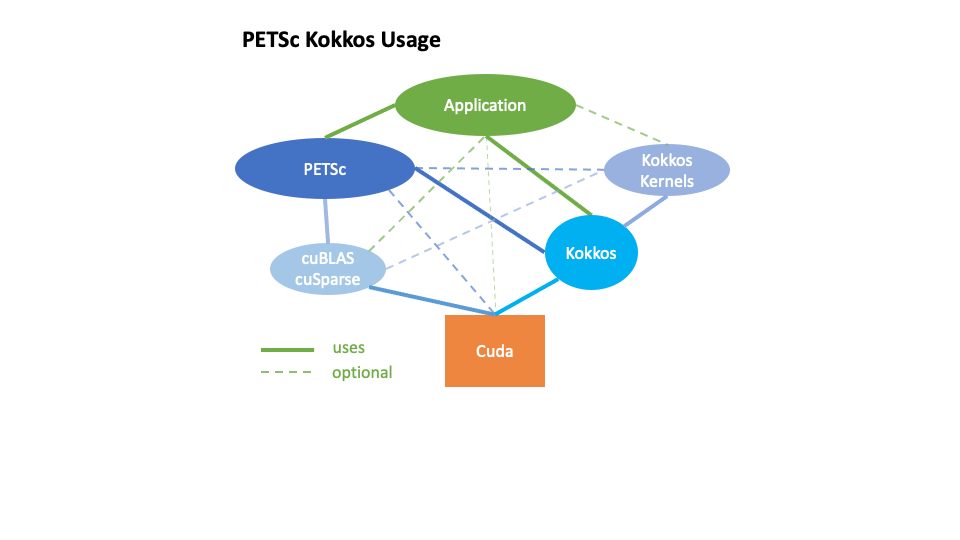
\includegraphics[trim = 2.8in 1.8in 2.8in .3in, clip, width=.79\linewidth]{PETSc-backends-kokkos-cuda.png}
\caption{Application using PETSc/Kokkos for CUDA system}
\label{fig:petsc_backends-kokkos}
\end{center}
\end{figure}

Cuda is the most mature target to date and Figure \ref{fig:petsc_backends-kokkos} sketches the composition of the two available back-ends.
One built on cuSparse and one built on Kokkos kernels with either Kokkos or cuSparse kernels.
All solvers share the same MPI layer.
Figure \ref{fig:gamg_weak_scaling} shows times for the solve phase as a function of the number Summit nodes, keeping the same number of cells per MPI task, that is weak scaling where  horizontal lines are perfect.
However the iteration count does increase by about 5\% within each data set as the global problem size increases and we thus do not quite have perfect algorithmic scaling.
We show data for several levels of refinement (local subdomain size), using the cuSparse back-end and the Kokkos kernels back-end using Kokkos's kernels (ie, not using the ``third party libraries" Kokkos configuration, but we have observed the performance is similar).
\begin{figure}[htbp]
\begin{center}
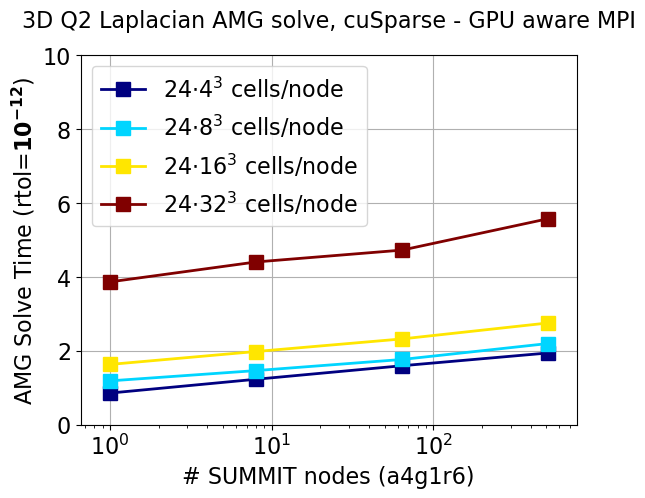
\includegraphics[width=.49\linewidth]{weak_scaling_cuda_def_a4g1r6.png}
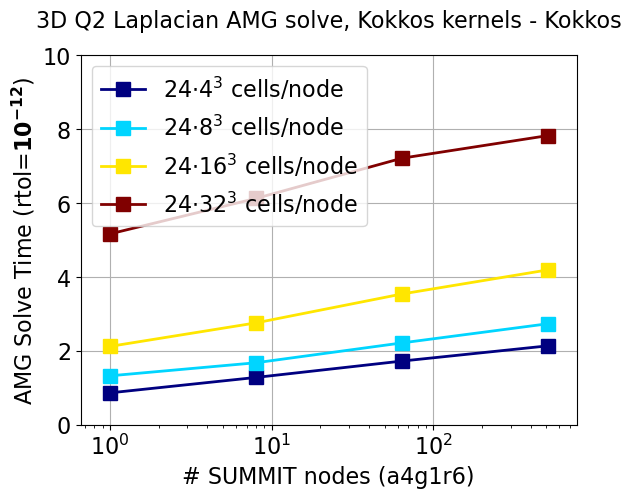
\includegraphics[width=.49\linewidth]{weak_scaling_kokkos_notpl_a4g1r6.png}
% can make 2x bigger and stack -- change caption accordingly
\caption{Solve time (sec) for 10 solves of a 3D Laplacian on Summit with cuSparse (top) and Kokkos kernels (bottom) back-ends, with a relative residual tolerance of $10^{-12}$ and six  'resource sets' on each node, each with one GPUs and 4 MPI processes}
\label{fig:gamg_weak_scaling}
\end{center}
\end{figure}

These tests uses Q2 elements, 10 solves with a relative residual tolerance of $10^{-12}$, and keep a logical cube of cells one each MPI process, with 24 cores per Summit node (ie, 4 MPI tasks per GPU).
The four refinement levels simply refine by a factor of two in each dimension from a base case of $4^3$ cell grid.
This data shows that the Kokkos kernels and cuSparse back-ends are performing comparably.
This data indicates that these two back-ends (cuSparse and Kokkos-kernels) are reasonably well optimized, or are at least optimized to a similar degree, and the common MPI layer is scaling reasonably well on Summit.

%\bibliography{mybibfile}

\end{document}
